\chapter{合成：产率与纯度}\label{ch:g10:synthesis-yield}

阿司匹林是世界上使用最广泛的药物之一。它的故事始于柳树皮，
人们很早就嚼食柳树皮以止痛退热。十九世纪，树皮中的有效成分
被追溯为一类化合物，化学家由此制得水杨酸。
水杨酸对胃刺激过强，不宜大剂量服用，于是人们将其改造为
较温和的乙酰水杨酸，即阿司匹林。
如今，它在钢制反应釜中按吨生产，所用反应与学校实验室里
一个下午即可完成的反应相同。
制备物质只是工作的一半，还必须将它与烧瓶中的其他物质分离，
并加以提纯、检验，
再称量，以确定
实际得到了多少预期产物。

\begin{recall}
回顾：萃取、\omterm{def:g10:chemical-species:distillation}{蒸馏}、\omterm{def:g10:chemical-species:tlc}{薄层色谱法}和\omterm{def:g10:chemical-species:retention-factor}{比移值}；
纯净固体在一个尖锐而确定的温度下熔化
（见\cref{ch:g10:chemical-species}）。\omterm{def:g3:separating-mixtures:filter}{过滤}可截留固体，使液体通过
（见\cref{ch:g3:separating-mixtures}）。\omterm{def:g10:reaction-progress-table:extent}{进度表}
给出\omterm{def:g10:reaction-progress-table:limiting}{限量反应物}所能得到的生成物的最大量
（见\cref{ch:g10:reaction-progress-table}）。
\end{recall}

\begin{omfigure}
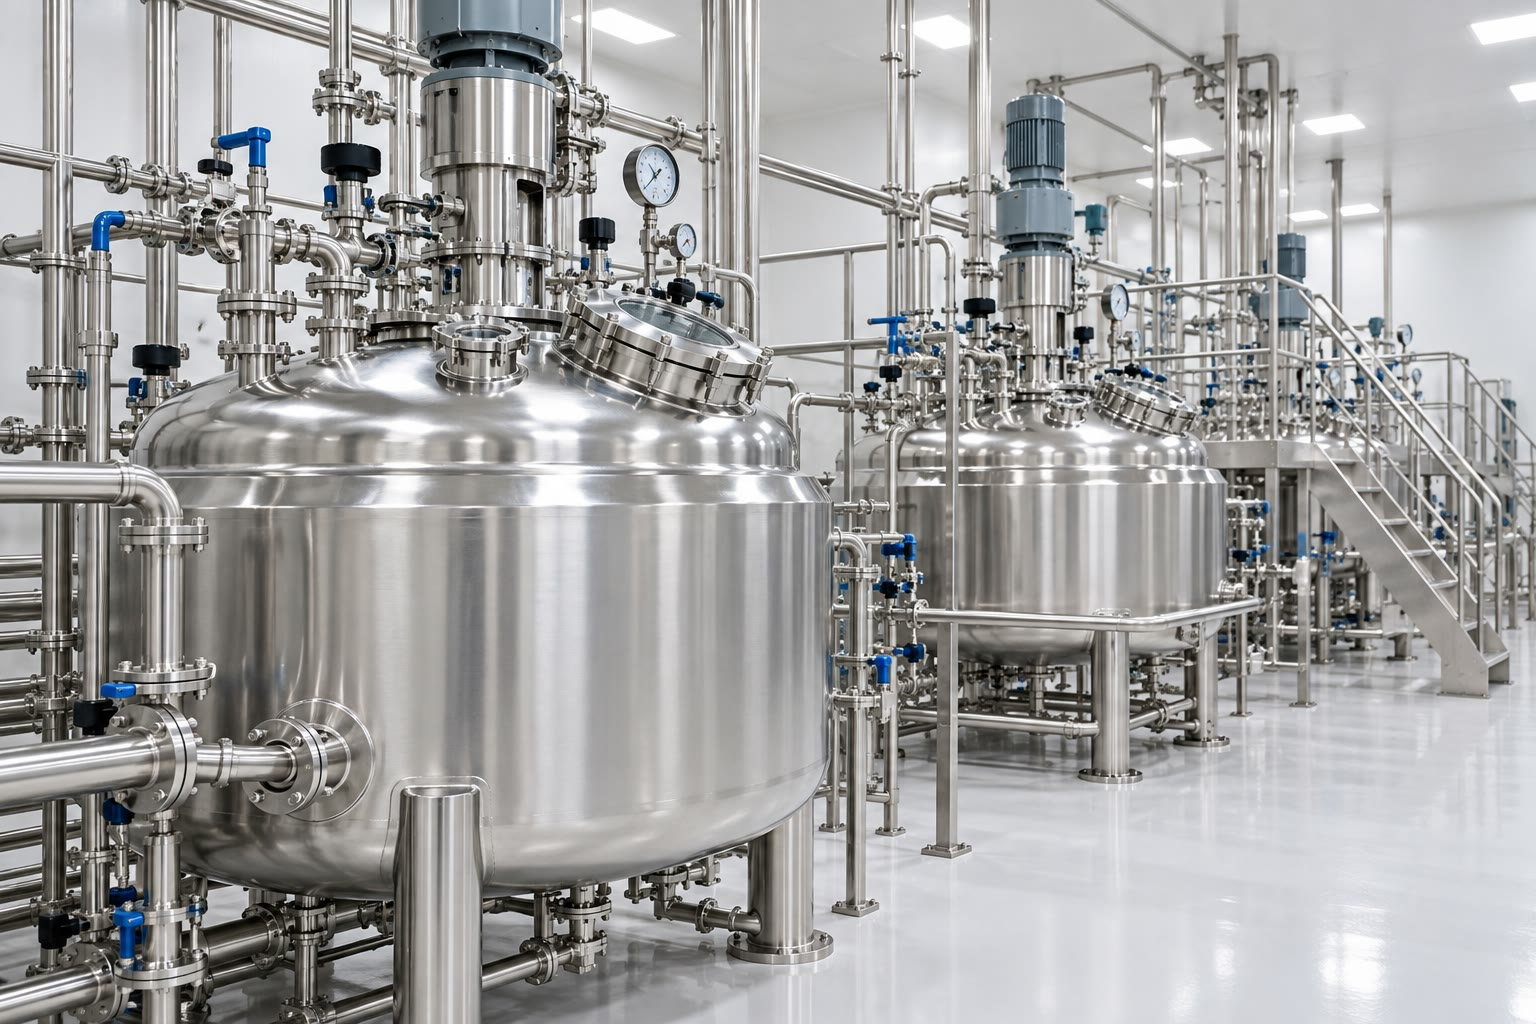
\includegraphics[width=0.55\linewidth]{images/book1/ai/g10-pharma-reactor.jpg}

{\small 制药厂中的钢制反应釜：实验室里的\omterm{def:g10:synthesis-yield:synthesis}{合成}，
规模放大了一百万倍。}
\end{omfigure}

\section{合成的步骤}

\begin{definition}[合成，粗产物]\label{def:g10:synthesis-yield:synthesis}
称\emph{合成}\index{合成}为由其他物种出发，
经一步或多步\omterm{def:g7:chemical-reactions:reaction}{化学反应}制备\omterm{def:g6:pure-substances-and-mixtures:species}{化学物种}的过程。
从反应\omterm{def:g6:pure-substances-and-mixtures:mixture}{混合物}中直接回收的、未经任何提纯的
固体或液体，称为\emph{粗产物}\index{粗产物}，
其中仍含有\omterm{def:g7:chemical-reactions:reactant}{反应物}、副产物
和\omterm{def:g6:solutions-and-solubility:solute}{溶剂}。
\end{definition}

\begin{method}[设计合成方案]\label{met:g10:synthesis-yield:plan}
\omterm{def:g10:synthesis-yield:synthesis}{合成}分四步进行：
\begin{enumerate}
  \item \textbf{反应}：按适当的用量\omterm{def:g2:mixing-and-dissolving:mix}{混合}\omterm{def:g7:chemical-reactions:reactant}{反应物}，常使其中一种过量，
        必要时加热。
  \item \textbf{分离}：将\omterm{def:g10:synthesis-yield:synthesis}{粗产物}与反应\omterm{def:g6:pure-substances-and-mixtures:mixture}{混合物}分开
        （\omterm{def:g3:separating-mixtures:filter}{过滤}、萃取）。
  \item \textbf{提纯}：除去\omterm{def:g10:synthesis-yield:synthesis}{粗产物}中的杂质，
        固体常用\omterm{def:g10:synthesis-yield:recrystallisation}{重结晶}，
        液体常用\omterm{def:g10:chemical-species:distillation}{蒸馏}。
  \item \textbf{分析}：鉴定产物的组成与纯度
        （熔点、色谱法），然后称量并
        计算\omterm{def:g10:synthesis-yield:yield}{产率}。
\end{enumerate}
\end{method}

\begin{example}[制备阿司匹林]\label{ex:g10:synthesis-yield:aspirin}
水杨酸与乙酸酐（又称醋酸酐）反应，
生成阿司匹林和乙酸：
\[
  \ce{C7H6O3 + C4H6O3 -> C9H8O4 + C2H4O2}
\]
\[
  \text{水杨酸} + \text{乙酸酐} \longrightarrow
  \text{阿司匹林} + \text{乙酸}.
\]
乙酸酐过量加入，以使水杨酸全部反应；
生成的乙酸是副产物。
\end{example}

\begin{omfigure}
\setchemfig{atom sep=1.7em}
\begin{tabular}{@{}c@{\enspace}c@{\enspace}c@{\enspace}c@{\enspace}c@{\enspace}c@{\enspace}c@{}}
\chemfig{*6(-=-(-COOH)=(-OH)-=)} & $+$ &
\chemfig{H_3C-C(=[2]O)-O-C(=[2]O)-CH_3} & $\longrightarrow$ &
\chemfig{*6(-=-(-COOH)=(-O-[:150]C(=[:90]O)-[:210]H_3C)-=)} & $+$ &
\chemfig{H_3C-C(=[2]O)-OH} \\[2pt]
\small 水杨酸 & & \small 乙酸酐 & &
\small 阿司匹林 & & \small 乙酸
\end{tabular}\par\medskip

{\small 阿司匹林的制备，以结构式表示（六边形的每个顶点
为一个碳\omterm{def:g7:atoms-and-molecules:atom}{原子}，凡未画出其他基团处均连有一个氢\omterm{def:g7:atoms-and-molecules:atom}{原子}；
后面的章节会解释这种简写）。水杨酸环上的\ce{-OH}
基团与一半乙酸酐反应，
另一半则以乙酸的形式离去。}
\end{omfigure}

\section{加热回流}

\begin{definition}[加热回流]\label{def:g10:synthesis-yield:reflux}
称\emph{加热回流}\index{加热回流}为在顶端装有竖直冷凝器的烧瓶中
加热反应\omterm{def:g6:pure-substances-and-mixtures:mixture}{混合物}：蒸气上升，在冷凝器中冷却，
液体流回烧瓶中。
\end{definition}

\begin{proposition}[为什么要回流]\label{prop:g10:synthesis-yield:why-reflux}
加热能使大多数反应加快；回流使人们能够在\omterm{def:g6:pure-substances-and-mixtures:mixture}{混合物}的沸点温度下
按需要长时间加热，而不会使任何\omterm{def:g7:chemical-reactions:reactant}{反应物}、生成物或\omterm{def:g6:solutions-and-solubility:solute}{溶剂}
以蒸气的形式损失。
\end{proposition}

\begin{proof}
沸腾液体的温度不可能超过其沸点，
而每一份从液体中逸出的蒸气都会被冷凝并送回：
装置中没有任何物质逸出，装置顶部保持敞开，
以免压强升高。
\end{proof}

\begin{omfigure}
\begin{tikzpicture}[font=\small, scale=1.05]
  \pic[transform shape] at (0,0) {heatingmantle};
  \pic[transform shape] at (0,0) {rbflask={0.42}{orange!25}};
  \foreach \p in {(-0.3,0.25), (0.2,0.18), (0.45,0.4), (-0.5,0.5)}
    \fill[black!45] \p circle (0.05);
  \pic[transform shape] at (0,3.0) {condenser};
  \draw[omDef, thick, <-] (0.8,3.825) -- (1.9,3.825) node[right] {进水};
  \draw[omDef, thick, ->] (0.8,5.375) -- (1.9,5.375) node[right] {出水};
  \draw[omProp, thick, <-] (-0.18,5.8) -- (-1.4,6.1) node[left] {顶部开口};
  \draw[omProp, thick, <-] (-0.45,1.2) -- (-2.0,1.6)
    node[left, align=right] {反应混合物 \\ 和沸石};
  \draw[omProp, thick, <-] (-1.35,-0.2) -- (-2.0,-0.6)
    node[left] {加热套};
  \draw[omThm, ->, thick] (-0.05,3.4) -- (-0.05,4.3);
  \draw[omDef, ->, thick] (0.05,4.3) -- (0.05,3.4);
  \node[omThm, anchor=east, font=\footnotesize] at (-0.45,4.6) {蒸气上升};
  \node[omDef, anchor=west, font=\footnotesize] at (0.85,4.6) {液体回落};
\end{tikzpicture}

{\small \omterm{def:g10:synthesis-yield:reflux}{加热回流}。冷水由冷凝器底部进入夹套，
从顶部流出，使夹套
始终充满。}
\end{omfigure}

\begin{remark}[底部进水]\label{rem:g10:synthesis-yield:water}
若从顶部进水，水将直接向下流走，使
夹套上部充满\omterm{def:g4:air-a-mixture-of-gases:air}{空气}；若从底部进水，水必须
充满整个夹套后才能流出。
\end{remark}

\section{分离与提纯}

\begin{definition}[减压过滤]\label{def:g10:synthesis-yield:vacuum-filtration}
称\emph{减压过滤}\index{减压过滤}为一种\omterm{def:g3:separating-mixtures:filter}{过滤}方式，
其中液体借助抽吸穿\omterm{def:g3:separating-mixtures:filter}{过滤}纸：
将带孔板的平底漏斗（布氏漏斗）置于
与真空泵相连的侧管抽滤瓶上。
\end{definition}

\begin{omfigure}
\begin{tikzpicture}[font=\small, scale=1.05]
  \pic[transform shape] (ff) at (0,0) {filterflask={0.12}{orange!20}};
  \fill[black!50] (-0.3,2.45) rectangle (0.3,2.8);
  \pic[transform shape] at (0,2.45) {buchner={black!8}};
  \draw[black!60, line width=2pt] (ff-arm) -- (2.6,2.2);
  \draw[omProp, thick, ->] (2.7,2.2) -- (3.4,2.2) node[right,
    align=left, text=black] {通向 \\ 真空泵};
  \draw[omProp, thick, <-] (0.7,3.8) -- (1.9,4.3) node[right, text=black]
    {滤纸上的晶体};
  \draw[omProp, thick, <-] (-0.4,0.15) -- (-1.8,0.6) node[left, text=black]
    {滤液};
  \draw[omProp, thick, <-] (-0.3,2.6) -- (-1.8,2.9) node[left, text=black]
    {橡胶密封圈};
\end{tikzpicture}

{\small 布氏漏斗\omterm{def:g10:synthesis-yield:vacuum-filtration}{减压过滤}：真空泵将
液体迅速抽过，并使固体几乎干燥。}
\end{omfigure}

\begin{definition}[重结晶]\label{def:g10:synthesis-yield:recrystallisation}
\emph{重结晶}\index{重结晶}是一种提纯固体的方法：
先将其溶于尽可能少的热\omterm{def:g6:solutions-and-solubility:solute}{溶剂}中，
再使溶液冷却：产物在冷时\omterm{def:g6:solutions-and-solubility:solubility}{溶解度}小得多，
结晶，而含量较少的杂质
仍留在溶液中。
\end{definition}

\begin{method}[重结晶提纯固体]\label{met:g10:synthesis-yield:recrystallise}
\begin{enumerate}
  \item 选择\omterm{def:g6:solutions-and-solubility:solute}{溶剂}，使产物在热时
        极易\omterm{def:g2:mixing-and-dissolving:dissolve}{溶解}、冷时几乎不溶。
  \item 向粗固体中逐份加入热\omterm{def:g6:solutions-and-solubility:solute}{溶剂}，
        恰好全部\omterm{def:g2:mixing-and-dissolving:dissolve}{溶解}为止。
  \item 让溶液缓慢冷却，再放入冰浴中，
        析出晶体。
  \item 用\omterm{def:g10:synthesis-yield:vacuum-filtration}{减压过滤}收集晶体，并用少量
        冰冷\omterm{def:g6:solutions-and-solubility:solute}{溶剂}洗涤，然后干燥。
\end{enumerate}
\end{method}


\begin{omfigure}
\begin{tikzpicture}[font=\small]
  % 1. crude solid + a little hot solvent, on a hot plate
  \pic at (0,0.3) {hotplate};
  \pic at (0,0.3) {erlenmeyer={0.18}{orange!12}};
  \foreach \p in {(-0.4,0.42),(-0.15,0.38),(0.1,0.45),(0.35,0.4),(-0.3,0.55),(0.2,0.6)}
    \fill[brown!60] \p circle (0.06);
  \node[align=center, anchor=north] at (0,-0.15) {1. 粗固体，\\ 热溶剂};
  % 2. clear hot solution
  \pic at (3,0.3) {hotplate};
  \pic at (3,0.3) {erlenmeyer={0.22}{orange!12}};
  \node[align=center, anchor=north] at (3,-0.15) {2. 全部溶解，\\ 澄清且热};
  % 3. ice bath: crystals
  \fill[cyan!12, draw=black!40] (5.0,0) rectangle (7.0,1.2);
  \foreach \p in {(5.2,0.9),(6.75,1.0),(5.3,0.3),(6.8,0.25)}
    \draw[black!35, fill=white] \p ++(-0.12,-0.1) rectangle ++(0.24,0.2);
  \pic at (6,0.1) {erlenmeyer={0.2}{orange!8}};
  \foreach \x/\y in {-0.45/0.18,-0.25/0.15,0/0.2,0.25/0.15,0.45/0.2,-0.1/0.3,0.15/0.32,
                     -0.35/0.32,0.35/0.33}
    \fill[white, draw=black!55] (6+\x,0.1+\y) -- ++(0.07,0.06) -- ++(0.07,-0.06)
      -- ++(-0.07,-0.06) -- cycle;
  \node[align=center, anchor=north] at (6,-0.15) {3. 冰浴冷却，\\ 析出晶体};
  % 4. filter
  \pic at (9,0) {filterflask={0.12}{orange!12}};
  \pic at (9,2.45) {buchner={black!12}};
  \fill[black!50] (8.7,2.45) rectangle (9.3,2.8);
  \node[align=center, anchor=north] at (9,-0.15) {4. 减压过滤，\\ 冷洗、干燥};
\end{tikzpicture}

{\small \omterm{def:g10:synthesis-yield:recrystallisation}{重结晶}分四步进行。杂质始终\omterm{def:g2:mixing-and-dissolving:dissolve}{溶解}在冷\omterm{def:g6:solutions-and-solubility:solute}{溶剂}中，
并进入\omterm{def:g3:separating-mixtures:filter}{滤液}。}
\end{omfigure}

\begin{remark}[损失不可避免]\label{rem:g10:synthesis-yield:losses}
% ledger: sol:aspirin-25, sol:aspirin-37
即使在冷的条件下，\omterm{def:g6:solutions-and-solubility:solute}{溶剂}仍会\omterm{def:g2:mixing-and-dissolving:dissolve}{溶解}一部分产物。阿司匹林
在水中的\omterm{def:g6:solutions-and-solubility:solubility}{溶解度}约为 \qty{3.3}{g/L}（\qty{25}{\celsius}），
在 \qty{37}{\celsius} 时约为其三倍，温度越高\omterm{def:g2:mixing-and-dissolving:dissolve}{溶解}越多：每毫升
\omterm{def:g3:separating-mixtures:filter}{滤液}和洗涤水都会带走少量阿司匹林。
\omterm{def:g10:synthesis-yield:recrystallisation}{重结晶}以质量的损失换取纯度。
\end{remark}

\section{产物分析}

\begin{proposition}[纯度的两项检验]\label{prop:g10:synthesis-yield:checks}
在这些检验的限度内，\omterm{def:g10:synthesis-yield:synthesis}{合成}所得的固体为纯净的，当且仅当：
\begin{itemize}
  \item 它在表中给出的熔点处明显熔化；
  \item 在薄层色谱板上，它只呈现一个斑点，
        与\omterm{def:g6:pure-substances-and-mixtures:pure-substance}{纯净物}样品的高度相同。
\end{itemize}
\end{proposition}

\begin{proof}
在本阶段不加证明地承认：杂质会降低熔点，并使熔化
发生在一个范围内（\cref{ch:g10:chemical-species}），而第二种物质通常
在色谱板上移动的距离不同。
\end{proof}

\begin{omfigure}
\begin{tikzpicture}[font=\small, scale=1.3]
  \pic[transform shape] at (0,0) {tlcplate};
  \draw[black!50, dashed] (-0.7,2.7) -- (0.7,2.7);
  % lanes: C crude, R recrystallised, A aspirin, S salicylic acid
  \foreach \x/\l in {-0.5/C,-0.17/R,0.17/A,0.5/S}
    \node[font=\footnotesize, anchor=north] at (\x,0.38) {\l};
  \fill[omDef!70] (-0.5,1.75) ellipse (0.09 and 0.06);
  \fill[omDef!40] (-0.5,1.25) ellipse (0.09 and 0.06);
  \fill[omDef!70] (-0.17,1.75) ellipse (0.09 and 0.06);
  \fill[omDef!70] (0.17,1.75) ellipse (0.09 and 0.06);
  \fill[omDef!70] (0.5,1.25) ellipse (0.09 and 0.06);
  \node[anchor=west, font=\footnotesize] at (0.85,2.7) {溶剂前沿};
  \node[anchor=west, font=\footnotesize] at (0.85,0.4) {起始线};
\end{tikzpicture}

{\small \omterm{def:g10:synthesis-yield:synthesis}{粗产物}（C）与\omterm{def:g10:synthesis-yield:recrystallisation}{重结晶}产物（R）的\omterm{def:g7:identifying-substances:chromatography}{色谱图}，
并列纯阿司匹林（A）和水杨酸（S），在紫外线下观察。
\omterm{def:g10:synthesis-yield:synthesis}{粗产物}中仍含有水杨酸，
\omterm{def:g10:synthesis-yield:recrystallisation}{重结晶}产物中则不含。}
\end{omfigure}

\section{产率}

\begin{definition}[产率]\label{def:g10:synthesis-yield:yield}
\omterm{def:g10:synthesis-yield:synthesis}{合成}的\emph{产率}\index{产率}$\eta$ 是指
实际所得的纯净干燥产物的\omterm{def:g10:the-mole:amount}{物质的量}，与\omterm{def:g10:reaction-progress-table:limiting}{限量反应物}
所能给出的最大\omterm{def:g10:the-mole:amount}{物质的量}之比：
\[
  \eta = \frac{n_{\text{所得}}}{n_{\max}} ,
\]
通常以百分数表示。
\end{definition}

\begin{proposition}[由质量求产率]\label{prop:g10:synthesis-yield:masses}
由于所得\omterm{def:g10:the-mole:amount}{物质的量}与最大\omterm{def:g10:the-mole:amount}{物质的量}针对同一种产物，其\omterm{def:g10:the-mole:molar-mass}{摩尔
质量}为 $M$，因此\omterm{def:g10:synthesis-yield:yield}{产率}也等于质量之比：
\[
  \eta = \frac{m_{\text{所得}}}{m_{\max}},
  \qquad m_{\max} = n_{\max} \times M,
\]
其中 $n_{\max}$ 取自\omterm{def:g10:reaction-progress-table:extent}{进度表}中 $x = x_{\max}$ 处的值。
\end{proposition}

\begin{proof}
$m_{\text{所得}} / m_{\max} = (n_{\text{所得}} M) / (n_{\max} M)
= n_{\text{所得}} / n_{\max}$。
\end{proof}

\begin{example}[小规模合成的产率]\label{ex:g10:synthesis-yield:small}
% ledger: aw:C, aw:H, aw:O
\qty{1.38}{g} 水杨酸（$M = \qty{138.0}{g/mol}$），即
\qty{0.0100}{mol}，与过量的乙酸酐反应。阿司匹林的最大
\omterm{def:g10:the-mole:amount}{物质的量}为 \qty{0.0100}{mol}，即
$0.0100 \times 180.0 = \qty{1.80}{g}$。若得到 \qty{1.35}{g} 纯净干燥的
阿司匹林，则 $\eta = 1.35 / 1.80 = 0.75$，\omterm{def:g10:synthesis-yield:yield}{产率}为
\qty{75}{\percent}。
\end{example}

\begin{remark}[产率为何低于 100 \%]\label{rem:g10:synthesis-yield:below}
每一步都会有产物损失：粘在玻璃仪器上，\omterm{def:g2:mixing-and-dissolving:dissolve}{溶解}在
\omterm{def:g3:separating-mixtures:filter}{滤液}和洗涤液中，或残留在\omterm{def:g10:synthesis-yield:recrystallisation}{重结晶}过程里；某些
反应还会生成副产物，或在\omterm{def:g10:reaction-progress-table:limiting}{限量反应物}
用尽之前便停止。\omterm{def:g10:synthesis-yield:yield}{产率}高于 \qty{100}{\percent} 总是提示
存在误差，最常见的原因是称量了仍湿润或含杂质的产物。
\end{remark}

\begin{inthelab}[制备阿司匹林]
教师在干燥的烧瓶中，将水杨酸与过量的
乙酸酐及几滴能加快反应的酸\omterm{def:g2:mixing-and-dissolving:mix}{混合}，
并在水浴中\omterm{def:g10:synthesis-yield:reflux}{加热回流}，温度约
\qty{80}{\celsius} 下持续十五分钟。冷却后，
加入冷水：过量的乙酸酐与水反应，而几乎不溶于冷水的
阿司匹林以白色晶体析出。这些晶体须
经\omterm{def:g10:synthesis-yield:vacuum-filtration}{减压过滤}收集，再经\omterm{def:g10:synthesis-yield:recrystallisation}{重结晶}、干燥、称重，并测定其
熔点。
\end{inthelab}

\begin{safety}{\ghs[0.82cm]{GHS02}\ghs[0.82cm]{GHS05}\ghs[0.82cm]{GHS06}\ghs[0.82cm]{GHS07}}
% ledger: ghs:acetic-anhydride, ghs:salicylic, ghs:aspirin
乙酸酐易燃，吞食或吸入有害，并会严重灼伤
皮肤和眼睛：须由教师在通风橱中操作，
并佩戴手套和护目镜。水杨酸吞食有害，并
可能损伤眼睛。实验室制得的阿司匹林绝不可
作为药物服用。
\end{safety}

\begin{omfigure}
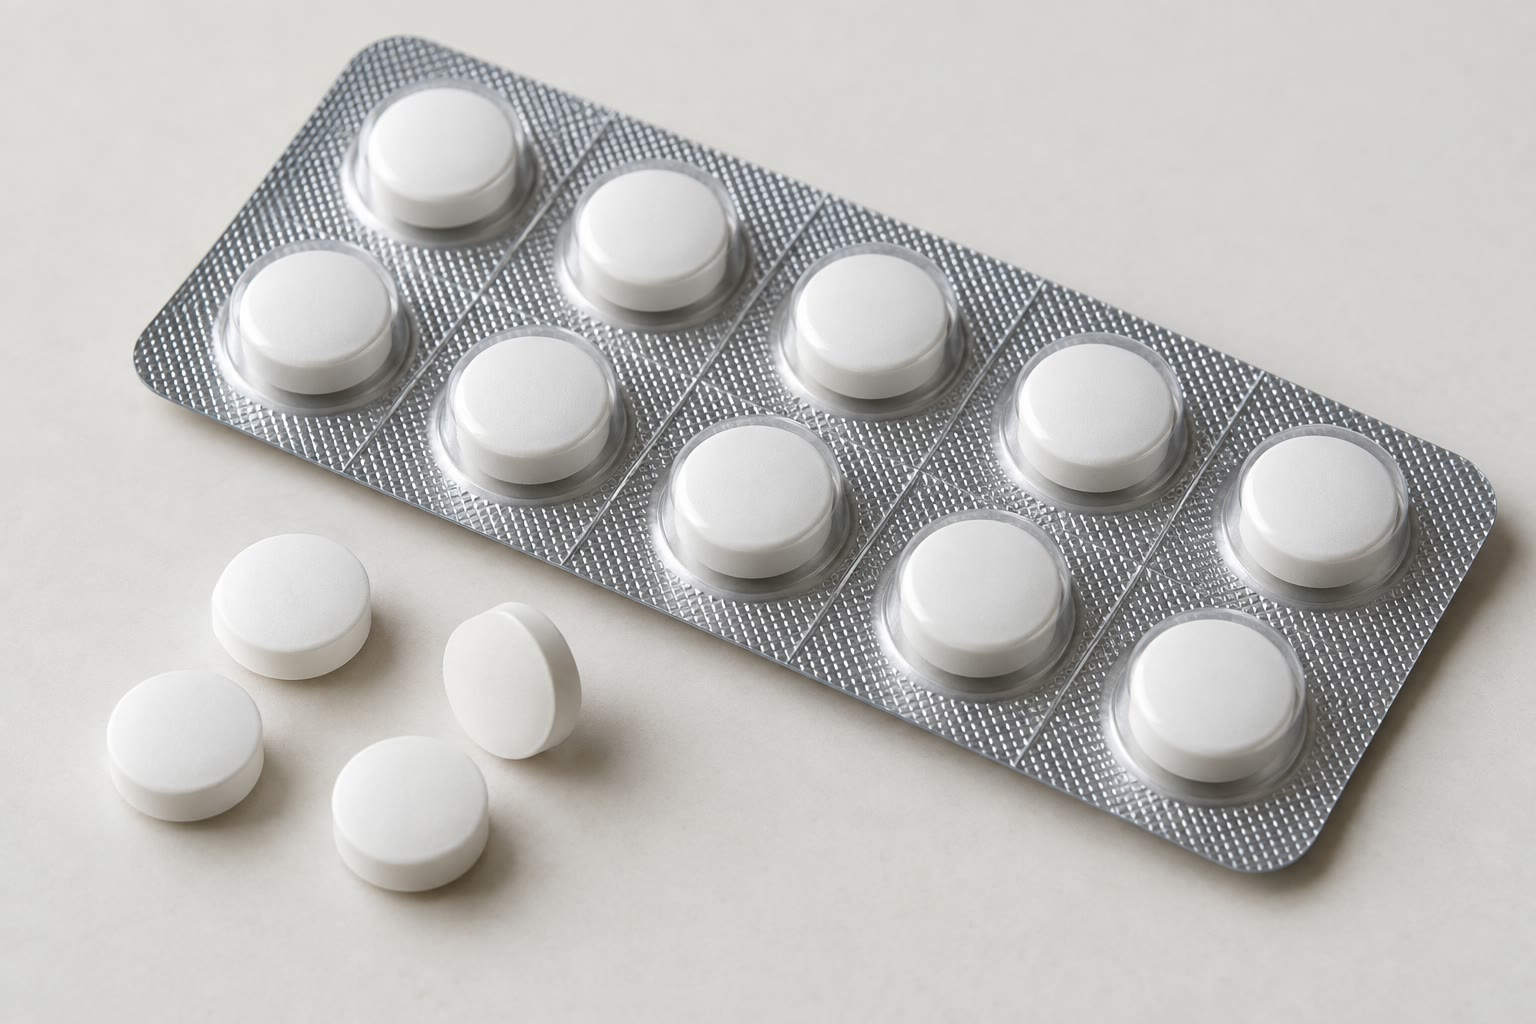
\includegraphics[width=0.45\linewidth]{images/book1/ai/g10-aspirin-tablets.jpg}

{\small 阿司匹林片剂：每片含有称量好的\omterm{def:g6:pure-substances-and-mixtures:pure-substance}{纯净物}质，
与粘合剂\omterm{def:g2:mixing-and-dissolving:mix}{混合}。}
\end{omfigure}

\section{练习}


\begin{exercise}[$\star$]\label{exo:g10:synthesis-yield:1}
\omterm{def:g10:synthesis-yield:synthesis}{合成}反应最多可得 \qty{5.0}{g} 产物；实际得到 \qty{4.2}{g}
干燥的纯净产物。计算\omterm{def:g10:synthesis-yield:yield}{产率}。
\end{exercise}

\begin{exercise}[$\star$]\label{exo:g10:synthesis-yield:2}
按顺序排列该\omterm{def:g10:synthesis-yield:synthesis}{合成}的以下步骤：测定熔点；
\omterm{def:g10:synthesis-yield:reflux}{加热回流}；\omterm{def:g10:synthesis-yield:recrystallisation}{重结晶}；对\omterm{def:g10:synthesis-yield:synthesis}{粗产物}进行\omterm{def:g10:synthesis-yield:vacuum-filtration}{减压过滤}；
称量\omterm{def:g7:chemical-reactions:reactant}{反应物}。
\end{exercise}

\begin{exercise}[$\star$]\label{exo:g10:synthesis-yield:3}
在回流装置中，为什么要从冷凝器的下端通入冷却水？
冷凝器的上端为什么要保持敞开？
\end{exercise}

\begin{exercise}[$\star$]\label{exo:g10:synthesis-yield:4}
进行\omterm{def:g10:synthesis-yield:recrystallisation}{重结晶}时，\omterm{def:g6:solutions-and-solubility:solute}{溶剂}需要具备哪两种性质？杂质最终
会去向何处？
\end{exercise}

\begin{exercise}[$\star$]\label{exo:g10:synthesis-yield:5}
% ledger: mp:aspirin
某\omterm{def:g10:synthesis-yield:synthesis}{合成}阿司匹林样品的熔化区间为 \qty{124}{\celsius} 至
\qty{130}{\celsius} 之间。纯阿司匹林约在 \qty{135}{\celsius} 熔化。
该样品是否纯净？应如何处理？
\end{exercise}

\begin{exercise}[$\star\star$]\label{exo:g10:synthesis-yield:6}
\qty{2.00}{g} 水杨酸与过量的乙酸酐反应，
得到 \qty{2.03}{g} 干燥的纯阿司匹林。计算阿司匹林的
理论最大质量及\omterm{def:g10:synthesis-yield:yield}{产率}。
\end{exercise}

\begin{exercise}[$\star\star$]\label{exo:g10:synthesis-yield:7}
某学生在阿司匹林尚未干燥时称量，得到的\omterm{def:g10:synthesis-yield:yield}{产率}为
\qty{104}{\percent}。请解释原因。若称量未经提纯
但已干燥的\omterm{def:g10:synthesis-yield:synthesis}{粗产物}，所得\omterm{def:g10:synthesis-yield:yield}{产率}与真实\omterm{def:g10:synthesis-yield:yield}{产率}相比
是偏高还是偏低？
\end{exercise}

\begin{exercise}[$\star\star$]\label{exo:g10:synthesis-yield:8}
与用纸锥进行普通\omterm{def:g3:separating-mixtures:filter}{过滤}相比，收集晶体时
\omterm{def:g10:synthesis-yield:vacuum-filtration}{减压过滤}有哪两个优点？
\end{exercise}

\begin{exercise}[$\star\star$]\label{exo:g10:synthesis-yield:9}
在色谱板上，\omterm{def:g6:solutions-and-solubility:solute}{溶剂}前沿移动了 \qty{5.0}{cm}。
\omterm{def:g10:synthesis-yield:synthesis}{合成}产物的斑点移动了 \qty{3.1}{cm}，
纯阿司匹林的斑点移动了 \qty{3.1}{cm}，水杨酸的斑点移动了 \qty{2.2}{cm}。
计算三种\omterm{def:g10:chemical-species:retention-factor}{比移值}。对产物可得出什么结论？
\end{exercise}

\begin{exercise}[$\star\star$]\label{exo:g10:synthesis-yield:10}
某产物在两种\omterm{def:g6:solutions-and-solubility:solute}{溶剂}中的\omterm{def:g6:solutions-and-solubility:solubility}{溶解度}如下：
\begin{center}
\begin{tabular}{lcc}
\hline
\omterm{def:g6:solutions-and-solubility:solute}{溶剂} & 冷（\qty{20}{\celsius}） & 热（接近沸点） \\
\hline
A & \qty{2}{g/L} & \qty{150}{g/L} \\
B & \qty{80}{g/L} & \qty{120}{g/L} \\
\hline
\end{tabular}
\end{center}
哪种\omterm{def:g6:solutions-and-solubility:solute}{溶剂}更适合用于\omterm{def:g10:synthesis-yield:recrystallisation}{重结晶}？对于 \qty{3.0}{g} \omterm{def:g10:synthesis-yield:synthesis}{粗产物}，
大约需要多少体积的热\omterm{def:g6:solutions-and-solubility:solute}{溶剂}，冷却后最多有多少质量
仍\omterm{def:g2:mixing-and-dissolving:dissolve}{溶解}在溶液中？
\end{exercise}

\begin{exercise}[$\star\star$]\label{exo:g10:synthesis-yield:11}
为什么回流装置中的圆底烧瓶绝不会装得超过
一半？为什么要加入沸石？
\end{exercise}

\begin{exercise}[$\star\star\star$]\label{exo:g10:synthesis-yield:12}
某药物分两步\omterm{def:g10:synthesis-yield:synthesis}{合成}，两步的\omterm{def:g10:synthesis-yield:yield}{产率}分别为 \qty{80}{\percent} 和
\qty{70}{\percent}。总\omterm{def:g10:synthesis-yield:yield}{产率}是多少？若三步反应的\omterm{def:g10:synthesis-yield:yield}{产率}各为 \qty{90}{\percent}，
总\omterm{def:g10:synthesis-yield:yield}{产率}又是多少？化学家为何要尽量减少
药物\omterm{def:g10:synthesis-yield:synthesis}{合成}的步骤数？
\end{exercise}

\begin{exercise}[$\star\star\star$]\label{exo:g10:synthesis-yield:13}
% ledger: sol:aspirin-25
阿司匹林在水中的\omterm{def:g6:solutions-and-solubility:solubility}{溶解度}（\qty{25}{\celsius}）约为
\qty{3.3}{g/L}。晶体用 \qty{50}{mL} 该温度下的水洗涤。
最多可能损失多少质量的阿司匹林？
为什么洗涤用水要先用冰冷却？
\end{exercise}

\begin{exercise}[$\star\star\star$]\label{exo:g10:synthesis-yield:14}
\qty{2.76}{g} 水杨酸与 \qty{0.0500}{mol}
乙酸酐\omterm{def:g2:mixing-and-dissolving:mix}{混合}。反应结束后，加入水以破坏
过量的酸酐：\ce{C4H6O3 + H2O -> 2C2H4O2}。
\begin{enumerate}
  \item 填写\omterm{def:g10:synthesis-yield:synthesis}{合成}反应的\omterm{def:g10:reaction-progress-table:extent}{进度表}；剩余酸酐的\omterm{def:g10:the-mole:amount}{物质的量}
        为多少？
  \item 反应结束时，体系中乙酸的\omterm{def:g10:the-mole:amount}{物质的量}共为多少？
\end{enumerate}
\end{exercise}

\begin{exercise}[$\star\star\star$]\label{exo:g10:synthesis-yield:15}
某工厂要生产 \qty{1.00}{t} 阿司匹林，以水杨酸计，总\omterm{def:g10:synthesis-yield:yield}{产率}为
\qty{85}{\percent}。该厂需购入水杨酸的
质量为多少？
\end{exercise}

\section{问题：制备阿司匹林}

\begin{problem}[{周末问题——从三克水杨酸
制得一瓶纯阿司匹林：产率是多少？}]
\label{pb:g10:synthesis-yield:1}
% ledger: rho:acetic-anhydride, mp:aspirin, mp:salicylic, sol:aspirin-25, aw:C, aw:H, aw:O
某班级制备阿司匹林。烧瓶中加入 \qty{3.0}{g} 水杨酸和
\qty{6.0}{mL} 乙酸酐（密度为 \qty{1.08}{g/mL}），并加入
几滴酸，将\omterm{def:g6:pure-substances-and-mixtures:mixture}{混合物}\omterm{def:g10:synthesis-yield:reflux}{加热回流}。\omterm{def:g10:synthesis-yield:synthesis}{粗产物}经\omterm{def:g10:synthesis-yield:vacuum-filtration}{减压过滤}收集，湿重
\qty{3.6}{g}，干重 \qty{3.3}{g}。\omterm{def:g10:synthesis-yield:recrystallisation}{重结晶}并干燥后，得到
\qty{2.7}{g} 白色晶体。
%

\medskip
\noindent\textbf{第一部分——反应。}
\begin{enumerate}
  \item 检验下列方程式
        \ce{C7H6O3 + C4H6O3 -> C9H8O4 + C2H4O2} 是否配平。
  \item 计算水杨酸、乙酸酐、
        阿司匹林和乙酸的\omterm{def:g10:the-mole:molar-mass}{摩尔质量}。
  \item 写出\omterm{def:g7:chemical-reactions:reactant}{反应物}、目标产物和副产物的名称。
  \item 为何\omterm{def:g6:pure-substances-and-mixtures:mixture}{混合物}要\omterm{def:g10:synthesis-yield:reflux}{加热回流}，而不在
        敞口烧瓶中加热？
\end{enumerate}

\medskip
\noindent\textbf{第二部分——最大质量。}
\begin{enumerate}[resume]
  \item 计算水杨酸的初始\omterm{def:g10:the-mole:amount}{物质的量}。
  \item 计算乙酸酐的质量，再计算其\omterm{def:g10:the-mole:amount}{物质的量}。
  \item 填写\omterm{def:g10:reaction-progress-table:extent}{进度表}。哪种\omterm{def:g7:chemical-reactions:reactant}{反应物}为\omterm{def:g10:reaction-progress-table:limiting}{限量反应物}？
        给出 $x_{\max}$。
  \item 推算阿司匹林的最大质量。
  \item 为何过量加入的是乙酸酐，而
        不是水杨酸？
\end{enumerate}

\medskip
\noindent\textbf{第三部分——分离与提纯。}
\begin{enumerate}[resume]
  \item 为何不能用湿重 \qty{3.6}{g} 计算
        \omterm{def:g10:synthesis-yield:yield}{产率}？
  \item 计算\omterm{def:g10:synthesis-yield:synthesis}{粗产物}干品的\omterm{def:g10:synthesis-yield:yield}{产率}。
  \item 为何\omterm{def:g10:synthesis-yield:recrystallisation}{重结晶}会使质量降低？
  \item 用 \qty{30}{mL} 水洗涤晶体，水温为
        \qty{25}{\celsius}，此时阿司匹林的\omterm{def:g6:solutions-and-solubility:solubility}{溶解度}约为
        \qty{3.3}{g/L}。这样最多会损失多少质量？
  \item 计算纯产物的\omterm{def:g10:synthesis-yield:yield}{产率}。
\end{enumerate}

\medskip
\noindent\textbf{第四部分——检验产物。}
\begin{enumerate}[resume]
  \item \omterm{def:g10:synthesis-yield:recrystallisation}{重结晶}后的晶体在 \qty{135}{\celsius}
        时熔化，熔程很窄。这说明什么？
  \item \omterm{def:g10:synthesis-yield:synthesis}{粗产物}在 \qty{120}{\celsius} 至
        \qty{131}{\celsius} 之间熔化。这说明什么？
  \item 在色谱板上，\omterm{def:g10:synthesis-yield:synthesis}{粗产物}显示两个斑点，
        一个与纯阿司匹林位于同一高度，另一个与
        水杨酸位于同一高度；\omterm{def:g10:synthesis-yield:recrystallisation}{重结晶}产物只有一个斑点，
        位于阿司匹林的高度。由此得出结论。
  \item \omterm{def:g10:synthesis-yield:recrystallisation}{重结晶}产物的斑点移动了 \qty{3.1}{cm}，
        \omterm{def:g6:solutions-and-solubility:solute}{溶剂}前沿移动了 \qty{5.0}{cm}。计算其\omterm{def:g10:chemical-species:retention-factor}{比移值}。
  \item 在反应与\omterm{def:g10:synthesis-yield:recrystallisation}{重结晶}两个步骤中，哪一步
        损失阿司匹林更多？
  \item 给出最终答案：本次\omterm{def:g10:synthesis-yield:synthesis}{合成}的\omterm{def:g10:synthesis-yield:yield}{产率}是多少？
\end{enumerate}
\end{problem}
